\documentclass[12pt,a4paper]{article}
\usepackage{lmodern}

\usepackage{placeins}
\usepackage{amssymb,amsmath}
\usepackage{ifxetex,ifluatex}
\usepackage{fixltx2e} % provides \textsubscript
\ifnum 0\ifxetex 1\fi\ifluatex 1\fi=0 % if pdftex
  \usepackage[T1]{fontenc}
  \usepackage[utf8]{inputenc}
\else % if luatex or xelatex
  \ifxetex
    \usepackage{mathspec}
    \usepackage{xltxtra,xunicode}
  \else
    \usepackage{fontspec}
  \fi
  \defaultfontfeatures{Mapping=tex-text,Scale=MatchLowercase}
  \newcommand{\euro}{€}
\fi
% use upquote if available, for straight quotes in verbatim environments
\IfFileExists{upquote.sty}{\usepackage{upquote}}{}
% use microtype if available
\IfFileExists{microtype.sty}{%
\usepackage{microtype}
\UseMicrotypeSet[protrusion]{basicmath} % disable protrusion for tt fonts
}{}
\usepackage[lmargin = 2cm, rmargin = 2.5cm, tmargin = 2cm, bmargin = 2.5cm]{geometry}


% Figure Placement:
\usepackage{float}
\let\origfigure\figure
\let\endorigfigure\endfigure
\renewenvironment{figure}[1][2] {
    \expandafter\origfigure\expandafter[H]
} {
    \endorigfigure
}

%%%% Jens %%%%
\usepackage{titlesec}
\DeclareMathOperator*{\argmax}{arg\,max}
\DeclareMathOperator*{\argmin}{arg\,min}
\renewcommand{\vec}{\operatorname{vec}}
\newcommand{\tr}{\operatorname{tr}}
\newcommand{\Var}{\operatorname{Var}}
\newcommand{\Cov}{\operatorname{Cov}}



\titleformat{\section}
{\normalfont\large\bfseries}{\thesection}{1em}{}

\newcommand{\tmpsection}[1]{}
\let\tmpsection=\section
\renewcommand{\section}[1]{\tmpsection{\underline{#1}} }





%% citation setup
\usepackage{csquotes}

\usepackage[backend=biber, maxbibnames = 99, style = apa]{biblatex}
\setlength\bibitemsep{1.5\itemsep}
\addbibresource{R_packages.bib}
\usepackage{color}
\usepackage{fancyvrb}
\newcommand{\VerbBar}{|}
\newcommand{\VERB}{\Verb[commandchars=\\\{\}]}
\DefineVerbatimEnvironment{Highlighting}{Verbatim}{commandchars=\\\{\}}
% Add ',fontsize=\small' for more characters per line
\usepackage{framed}
\definecolor{shadecolor}{RGB}{248,248,248}
\newenvironment{Shaded}{\begin{snugshade}}{\end{snugshade}}
\newcommand{\AlertTok}[1]{\textcolor[rgb]{0.94,0.16,0.16}{#1}}
\newcommand{\AnnotationTok}[1]{\textcolor[rgb]{0.56,0.35,0.01}{\textbf{\textit{#1}}}}
\newcommand{\AttributeTok}[1]{\textcolor[rgb]{0.77,0.63,0.00}{#1}}
\newcommand{\BaseNTok}[1]{\textcolor[rgb]{0.00,0.00,0.81}{#1}}
\newcommand{\BuiltInTok}[1]{#1}
\newcommand{\CharTok}[1]{\textcolor[rgb]{0.31,0.60,0.02}{#1}}
\newcommand{\CommentTok}[1]{\textcolor[rgb]{0.56,0.35,0.01}{\textit{#1}}}
\newcommand{\CommentVarTok}[1]{\textcolor[rgb]{0.56,0.35,0.01}{\textbf{\textit{#1}}}}
\newcommand{\ConstantTok}[1]{\textcolor[rgb]{0.00,0.00,0.00}{#1}}
\newcommand{\ControlFlowTok}[1]{\textcolor[rgb]{0.13,0.29,0.53}{\textbf{#1}}}
\newcommand{\DataTypeTok}[1]{\textcolor[rgb]{0.13,0.29,0.53}{#1}}
\newcommand{\DecValTok}[1]{\textcolor[rgb]{0.00,0.00,0.81}{#1}}
\newcommand{\DocumentationTok}[1]{\textcolor[rgb]{0.56,0.35,0.01}{\textbf{\textit{#1}}}}
\newcommand{\ErrorTok}[1]{\textcolor[rgb]{0.64,0.00,0.00}{\textbf{#1}}}
\newcommand{\ExtensionTok}[1]{#1}
\newcommand{\FloatTok}[1]{\textcolor[rgb]{0.00,0.00,0.81}{#1}}
\newcommand{\FunctionTok}[1]{\textcolor[rgb]{0.00,0.00,0.00}{#1}}
\newcommand{\ImportTok}[1]{#1}
\newcommand{\InformationTok}[1]{\textcolor[rgb]{0.56,0.35,0.01}{\textbf{\textit{#1}}}}
\newcommand{\KeywordTok}[1]{\textcolor[rgb]{0.13,0.29,0.53}{\textbf{#1}}}
\newcommand{\NormalTok}[1]{#1}
\newcommand{\OperatorTok}[1]{\textcolor[rgb]{0.81,0.36,0.00}{\textbf{#1}}}
\newcommand{\OtherTok}[1]{\textcolor[rgb]{0.56,0.35,0.01}{#1}}
\newcommand{\PreprocessorTok}[1]{\textcolor[rgb]{0.56,0.35,0.01}{\textit{#1}}}
\newcommand{\RegionMarkerTok}[1]{#1}
\newcommand{\SpecialCharTok}[1]{\textcolor[rgb]{0.00,0.00,0.00}{#1}}
\newcommand{\SpecialStringTok}[1]{\textcolor[rgb]{0.31,0.60,0.02}{#1}}
\newcommand{\StringTok}[1]{\textcolor[rgb]{0.31,0.60,0.02}{#1}}
\newcommand{\VariableTok}[1]{\textcolor[rgb]{0.00,0.00,0.00}{#1}}
\newcommand{\VerbatimStringTok}[1]{\textcolor[rgb]{0.31,0.60,0.02}{#1}}
\newcommand{\WarningTok}[1]{\textcolor[rgb]{0.56,0.35,0.01}{\textbf{\textit{#1}}}}
\usepackage{graphicx}
\makeatletter
\def\maxwidth{\ifdim\Gin@nat@width>\linewidth\linewidth\else\Gin@nat@width\fi}
\def\maxheight{\ifdim\Gin@nat@height>\textheight\textheight\else\Gin@nat@height\fi}
\makeatother
% Scale images if necessary, so that they will not overflow the page
% margins by default, and it is still possible to overwrite the defaults
% using explicit options in \includegraphics[width, height, ...]{}
\setkeys{Gin}{width=\maxwidth,height=\maxheight,keepaspectratio}
\ifxetex
  \usepackage[setpagesize=false, % page size defined by xetex
              unicode=false, % unicode breaks when used with xetex
              xetex]{hyperref}
\else
  \usepackage[unicode=true, linktocpage = TRUE]{hyperref}
\fi
\hypersetup{breaklinks=true,
            bookmarks=true,
            pdfauthor={Dr.~Yannick Hoga},
            pdftitle={Multivariate Time Series Analysis},
            colorlinks=true,
            citecolor=black,
            urlcolor=black,
            linkcolor=black,
            pdfborder={0 0 0}}
\urlstyle{same}  % don't use monospace font for urls
\setlength{\parindent}{0pt}
\setlength{\parskip}{6pt plus 2pt minus 1pt}
\setlength{\emergencystretch}{3em}  % prevent overfull lines
\setcounter{secnumdepth}{5}

%%% Use protect on footnotes to avoid problems with footnotes in titles
\let\rmarkdownfootnote\footnote%
\def\footnote{\protect\rmarkdownfootnote}

%%% Change title format to be more compact
\usepackage{titling}

% Create subtitle command for use in maketitle
\newcommand{\subtitle}[1]{
  \posttitle{
    \begin{center}\large#1\end{center}
    }
}

\setlength{\droptitle}{-2em}
  \title{Multivariate Time Series Analysis}
  \pretitle{\vspace{\droptitle}\centering\huge}
  \posttitle{\par}
\subtitle{Exercise Sheet 2}
  \author{Dr.~Yannick Hoga}
  \preauthor{\centering\large\emph}
  \postauthor{\par}
  \date{}
  \predate{}\postdate{}


%% linespread settings

\usepackage{setspace}

\onehalfspacing


% Language Setup

\usepackage{ifthen}
\usepackage{iflang}
\usepackage[super]{nth}
\usepackage[ngerman, english]{babel}

%Acronyms
\usepackage[printonlyused, withpage, nohyperlinks]{acronym}
\usepackage{changepage}

% Multicols for the Title page
\usepackage{multicol}


% foot


\begin{document}

\selectlanguage{english}

%%%%%%%%%%%%%% Jens %%%%%
\numberwithin{equation}{section}




\restoregeometry


%%% Header 

\begin{minipage}{0.6\textwidth}
University of Duisburg-Essen\\
Faculty of Business Administration and Economics\\
Chair of Econometrics\\
\end{minipage}

%\begin{minipage}{0.4\textwidth}
	\begin{flushright}
	\vspace{-3cm}
	\includegraphics*[width=5cm]{Includes/duelogo_en.png}\\
	\vspace{.125cm}
	\end{flushright}
%\end{minipage}
%\vspace{.125cm}
\hspace{-0.005cm}Winter Term 2019/2020

\vspace{0.05cm}

\begin{center}
	\vspace{.25cm}
	Dr.~Yannick Hoga \hspace{.5cm} Thilo Reinschlüssel \\
	\vspace{.25cm}
	\textbf{\Large{Multivariate Time Series Analysis}}\\
	\vspace{.25cm}
	\textbf{\large{Exercise Sheet 2}}\\
	\vspace{.125cm}
\end{center}




% body from markdown

\hypertarget{exercise-1-moments-and-simulation-of-a-var1-process}{%
\section{Exercise 1: Moments and Simulation of a VAR(1)
Process}\label{exercise-1-moments-and-simulation-of-a-var1-process}}

Take the model from Example 2.4 on Slide 2-6:

\begin{itemize}
  \item[a)] Derive a formula to obtain the population cross-covariance matrices for the lags 1 to 10 and compute them using R.
  \item[] \textit{Hint: A glance at the slides and a loop might save you some time.}
  \item[b)] Based on your results, compute the cross-correlation matrices.
\end{itemize}

\emph{Solution:}\\

\begin{align*}
  z_t & = \phi_1 z_{t-1} + a_t\\
  \\
  \Gamma_0 & = \phi_1  \ \Gamma_0 \ \phi_1^{'} + \Sigma_a\\
  \Leftrightarrow \vec(\Gamma_0) &= (\phi_1 \otimes \phi_1) \cdot \vec(\Gamma_0) + \vec(\Sigma_a) \\
  \Leftrightarrow \vec(\Gamma_0) &= (I_{K^2} - \phi_1 \otimes \phi_1) \cdot \vec(\Sigma_a) \\
 \Rrightarrow \Gamma_1 & = \phi_1 \Gamma_0\\
 \Rrightarrow \Gamma_l & = \phi_{l-1} \Gamma_{l-1} = \phi_1^{l} \Gamma_0\\
\end{align*}

\begin{Shaded}
\begin{Highlighting}[]
\CommentTok{# First define parameters/coefficients:}
\NormalTok{Phi <-}\StringTok{ }\KeywordTok{matrix}\NormalTok{(}\DataTypeTok{data =} \KeywordTok{c}\NormalTok{(}\FloatTok{0.2}\NormalTok{, }\FloatTok{-0.6}\NormalTok{, }\FloatTok{0.3}\NormalTok{, }\FloatTok{1.1}\NormalTok{), }
              \DataTypeTok{byrow =} \OtherTok{FALSE}\NormalTok{, }\DataTypeTok{nrow =} \DecValTok{2}\NormalTok{) }\CommentTok{# VAR coefficients}
\NormalTok{k <-}\StringTok{ }\KeywordTok{ncol}\NormalTok{(Phi)}
\NormalTok{Sigma_a <-}\StringTok{ }\KeywordTok{matrix}\NormalTok{(}\DataTypeTok{data =} \KeywordTok{c}\NormalTok{(}\DecValTok{1}\NormalTok{, }\FloatTok{0.8}\NormalTok{, }\FloatTok{0.8}\NormalTok{, }\FloatTok{2.0}\NormalTok{), }
                  \DataTypeTok{byrow =} \OtherTok{FALSE}\NormalTok{, }\DataTypeTok{nrow =} \DecValTok{2}\NormalTok{) }\CommentTok{# innovations' covariances}

\NormalTok{Phi_kron <-}\StringTok{ }\KeywordTok{kronecker}\NormalTok{(}\DataTypeTok{X =}\NormalTok{ Phi, }\DataTypeTok{Y =}\NormalTok{ Phi) }\CommentTok{# kronecker product}
\CommentTok{# Phi %x% Phi # alternative command}

\NormalTok{Ident <-}\StringTok{ }\KeywordTok{diag}\NormalTok{(}\KeywordTok{ncol}\NormalTok{(Phi_kron)) }
\CommentTok{# identity matrix with the same dimensions as Phi_kron}

\NormalTok{Gamma0.vec <-}\StringTok{ }\KeywordTok{solve}\NormalTok{(Ident }\OperatorTok{-}\StringTok{ }\NormalTok{Phi_kron) }\OperatorTok\StringTok{ }\KeywordTok{c}\NormalTok{(Sigma_a) }
\CommentTok{# c() works like the "vec" operator}

\NormalTok{Gamma0.mat <-}\StringTok{ }\KeywordTok{matrix}\NormalTok{(}\DataTypeTok{data =}\NormalTok{ Gamma0.vec, }\DataTypeTok{nrow =} \DecValTok{2}\NormalTok{, }\DataTypeTok{byrow =} \OtherTok{FALSE}\NormalTok{)}
\end{Highlighting}
\end{Shaded}

The \(\Gamma_0\) matrix is than:

\begin{verbatim}
##          [,1]     [,2]
## [1,] 2.288889 3.511111
## [2,] 3.511111 8.622222
\end{verbatim}

To derive the \(\Gamma_1\) matrix, we can apply the following formula:

\begin{align*}
  \Gamma_1 & = \phi_1 \Gamma_0\\
\end{align*}

\begin{Shaded}
\begin{Highlighting}[]
\NormalTok{Gamma1.mat <-}\StringTok{ }\NormalTok{Phi }\OperatorTok\StringTok{ }\NormalTok{Gamma0.mat}
\end{Highlighting}
\end{Shaded}

\(\Gamma_1\) is than:

\begin{verbatim}
##          [,1]     [,2]
## [1,] 1.511111 3.288889
## [2,] 2.488889 7.377778
\end{verbatim}

To derive all desired \(l^{Th}\) laged covariance matrices we can use
the general equation and program a loop over all desired lags:

\begin{align*}
  \Rrightarrow \Gamma_l & = \phi_{l-1} \Gamma_{l-1} = \phi_1^{l} \Gamma_0\\
\end{align*}

To derive the correlation matrices \(\rho_l\) we devide the covariances
by the standard deviations:

\begin{align*}
  \rho_l = 
  \begin{pmatrix}
    \dfrac{\Cov(x_t , x_{t-l})}{\sqrt{\Var(x_t) \cdot \Var(x_{t- l})}} &
    \dfrac{cov(x_t , y_{t-l})}{\sqrt{\Var(x_t) \cdot \Var(y_{t- l})}}\\
    \dfrac{cov(y_t , x_{t-l})}{\sqrt{\Var(y_t) \cdot \Var(x_{t- l})}} &
    \dfrac{cov(y_t , y_{t-l})}{\sqrt{\Var(y_t) \cdot \Var(y_{t- l})}}
  \end{pmatrix}\\
\end{align*}

\begin{Shaded}
\begin{Highlighting}[]
\CommentTok{# compute further (lagged) cross-covariance-functions}
\CommentTok{# preparing the variables to store the matrices into: covariance}
\NormalTok{ccovf.list <-}\StringTok{ }\KeywordTok{list}\NormalTok{() }
\CommentTok{# """ : correlation}
\NormalTok{ccorf.list <-}\StringTok{ }\KeywordTok{list}\NormalTok{() }

\CommentTok{# obtaining standard deviations for the single variables (parts of z) }
\CommentTok{#and putting them in a diagonal matrix}
\NormalTok{D.inv <-}\StringTok{ }\KeywordTok{solve}\NormalTok{(}\KeywordTok{sqrt}\NormalTok{(Gamma0.mat }\OperatorTok{*}\StringTok{ }\KeywordTok{diag}\NormalTok{(}\KeywordTok{ncol}\NormalTok{(Phi)))) }
\ControlFlowTok{for}\NormalTok{ (i }\ControlFlowTok{in} \DecValTok{1}\OperatorTok{:}\DecValTok{10}\NormalTok{)\{}
\NormalTok{  ccovf.list[[i]] <-}\StringTok{ }\NormalTok{Phi}\OperatorTok\NormalTok{i }\OperatorTok\StringTok{ }\NormalTok{Gamma0.mat}
\NormalTok{  ccorf.list[[i]] <-}\StringTok{ }\NormalTok{D.inv }\OperatorTok\StringTok{ }\NormalTok{ccovf.list[[i]] }\OperatorTok\StringTok{ }\NormalTok{D.inv}
\NormalTok{\}}
\NormalTok{ccovf.list }\CommentTok{# cross lagged covariances}
\end{Highlighting}
\end{Shaded}

\begin{verbatim}
## [[1]]
##          [,1]     [,2]
## [1,] 1.511111 3.288889
## [2,] 2.488889 7.377778
## 
## [[2]]
##          [,1]     [,2]
## [1,] 1.048889 2.871111
## [2,] 1.831111 6.142222
## 
## [[3]]
##           [,1]     [,2]
## [1,] 0.7591111 2.416889
## [2,] 1.3848889 5.033778
## 
## [[4]]
##           [,1]     [,2]
## [1,] 0.5672889 1.993511
## [2,] 1.0679111 4.087022
## 
## [[5]]
##           [,1]     [,2]
## [1,] 0.4338311 1.624809
## [2,] 0.8343289 3.299618
## 
## [[6]]
##           [,1]     [,2]
## [1,] 0.3370649 1.314847
## [2,] 0.6574631 2.654694
## 
## [[7]]
##           [,1]     [,2]
## [1,] 0.2646519 1.059378
## [2,] 0.5209705 2.131255
## 
## [[8]]
##           [,1]      [,2]
## [1,] 0.2092215 0.8512522
## [2,] 0.4142764 1.7087543
## 
## [[9]]
##           [,1]      [,2]
## [1,] 0.1661272 0.6828767
## [2,] 0.3301711 1.3688784
## 
## [[10]]
##           [,1]      [,2]
## [1,] 0.1322768 0.5472389
## [2,] 0.2635119 1.0960403
\end{verbatim}

\begin{Shaded}
\begin{Highlighting}[]
\NormalTok{ccorf.list }\CommentTok{# cross lagged correlations}
\end{Highlighting}
\end{Shaded}

\begin{verbatim}
## [[1]]
##           [,1]      [,2]
## [1,] 0.6601942 0.7403332
## [2,] 0.5602522 0.8556701
## 
## [[2]]
##           [,1]      [,2]
## [1,] 0.4582524 0.6462909
## [2,] 0.4121855 0.7123711
## 
## [[3]]
##           [,1]      [,2]
## [1,] 0.3316505 0.5440449
## [2,] 0.3117403 0.5838144
## 
## [[4]]
##           [,1]      [,2]
## [1,] 0.2478447 0.4487420
## [2,] 0.2403882 0.4740103
## 
## [[5]]
##           [,1]      [,2]
## [1,] 0.1895379 0.3657466
## [2,] 0.1878085 0.3826876
## 
## [[6]]
##           [,1]      [,2]
## [1,] 0.1472614 0.2959738
## [2,] 0.1479958 0.3078898
## 
## [[7]]
##           [,1]      [,2]
## [1,] 0.1156246 0.2384673
## [2,] 0.1172711 0.2471817
## 
## [[8]]
##            [,1]      [,2]
## [1,] 0.09140746 0.1916180
## [2,] 0.09325416 0.1981803
## 
## [[9]]
##            [,1]      [,2]
## [1,] 0.07257985 0.1537165
## [2,] 0.07432195 0.1587617
## 
## [[10]]
##            [,1]      [,2]
## [1,] 0.05779083 0.1231842
## [2,] 0.05931687 0.1271181
\end{verbatim}

\begin{itemize}
  \item[c)] Draw a corresponding innovation sequence at for 300 periods from a (multivariate) Gaussian distribution and simulate the given VAR(1) process without any further built-in functions
  \item[] \textit{Hint: 'mvrnorm' and 'for' are still allowed}
\end{itemize}

\emph{Solution:}\\

\begin{enumerate}
  \item Set $T$ (in code $N$)
  \item Draw $\left\{ a_1, \ldots , a_T \right\} \sim \left[ \mu , \Sigma_a \right]$
  \item Set $z_0 = \mathbb{E} \left( z_t\right)$
  \item $z_1 = \phi_1 z_0 + a_1$
  \item Repeat Sep 4 $(T - 1)$ times
  \item (Discard first few observations to minimise effects of $z_0$ on the results)
  \begin{itemize}
    \item[$\Rightarrow$] \textit{Note} that it is generally advised to discard the first few observations to eliminate the influence of the arbitrary starting point! In our case we skipped this step to keep things short and clear.
  \end{itemize}
\end{enumerate}

\begin{Shaded}
\begin{Highlighting}[]
\CommentTok{# i) Set sample size and further coefficients}
\NormalTok{N <-}\StringTok{ }\DecValTok{300}
\CommentTok{# ii) The Basis: Innovations}
\KeywordTok{set.seed}\NormalTok{(}\DecValTok{2}\OperatorTok{^}\DecValTok{9-1}\NormalTok{) }\CommentTok{# for replication: the 'random' numbers drawn }
\CommentTok{# up from this point will always be the same (given you use }
\CommentTok{# the same command to draw them....)}
\NormalTok{a <-}\StringTok{ }\KeywordTok{mvrnorm}\NormalTok{(}\DataTypeTok{n =}\NormalTok{ N, }\DataTypeTok{mu =} \KeywordTok{c}\NormalTok{(}\DecValTok{0}\NormalTok{,}\DecValTok{0}\NormalTok{), }\DataTypeTok{Sigma =}\NormalTok{ Sigma_a)}
\CommentTok{# iii) Writing a function to generate 'z' realisations from 'a' using Phi}
\NormalTok{var1gen <-}\StringTok{ }\ControlFlowTok{function}\NormalTok{(coef.mat, z.lag, innovation)\{}
\NormalTok{  z.current <-}\StringTok{ }\NormalTok{coef.mat }\OperatorTok\StringTok{ }\NormalTok{z.lag }\OperatorTok{+}\StringTok{ }\NormalTok{innovation }
  \CommentTok{# z_(t) = phi * z_(t-1) + a_(t)}
  \KeywordTok{return}\NormalTok{(z.current)}
\NormalTok{\}}
\CommentTok{# iv) Prepare variable for 'z'}
\NormalTok{z <-}\StringTok{ }\KeywordTok{ts}\NormalTok{(}\DataTypeTok{data =} \KeywordTok{matrix}\NormalTok{(}\DataTypeTok{data =} \OtherTok{NA}\NormalTok{, }\DataTypeTok{nrow =}\NormalTok{ (N), }\DataTypeTok{ncol =}\NormalTok{ k)}
\NormalTok{        ,}\DataTypeTok{start =} \DecValTok{1}\NormalTok{, }\DataTypeTok{names =} \KeywordTok{c}\NormalTok{(}\StringTok{"z_1"}\NormalTok{, }\StringTok{"z_2"}\NormalTok{))}
\CommentTok{# v) Set starting values for z (at mean + innovation)}
\NormalTok{z[}\DecValTok{1}\NormalTok{,] <-}\StringTok{ }\KeywordTok{c}\NormalTok{(}\DecValTok{0}\NormalTok{,}\DecValTok{0}\NormalTok{) }\OperatorTok{+}\StringTok{ }\NormalTok{a[}\DecValTok{1}\NormalTok{,]}
\CommentTok{# vi) Generate z repeatedly and store it}
\ControlFlowTok{for}\NormalTok{ (i }\ControlFlowTok{in} \DecValTok{2}\OperatorTok{:}\NormalTok{(N))\{}
\NormalTok{  z[i,] <-}\StringTok{ }\KeywordTok{var1gen}\NormalTok{(}\DataTypeTok{coef.mat =}\NormalTok{ Phi, }\DataTypeTok{z.lag =}\NormalTok{ z[(i}\DecValTok{-1}\NormalTok{),], }\DataTypeTok{innovation =}\NormalTok{ a[i,])}
\NormalTok{\}}
\end{Highlighting}
\end{Shaded}

\begin{itemize}
  \item[d)] Plot the multivariate time series you have just created. Does it look stationary?
\end{itemize}

\begin{Shaded}
\begin{Highlighting}[]
\CommentTok{# The ordinary 'plot' command works because 'z' is already }
\CommentTok{# a 'ts'-class object (among other classes) and NOT a data frame!}
\KeywordTok{plot}\NormalTok{(z)}
\end{Highlighting}
\end{Shaded}

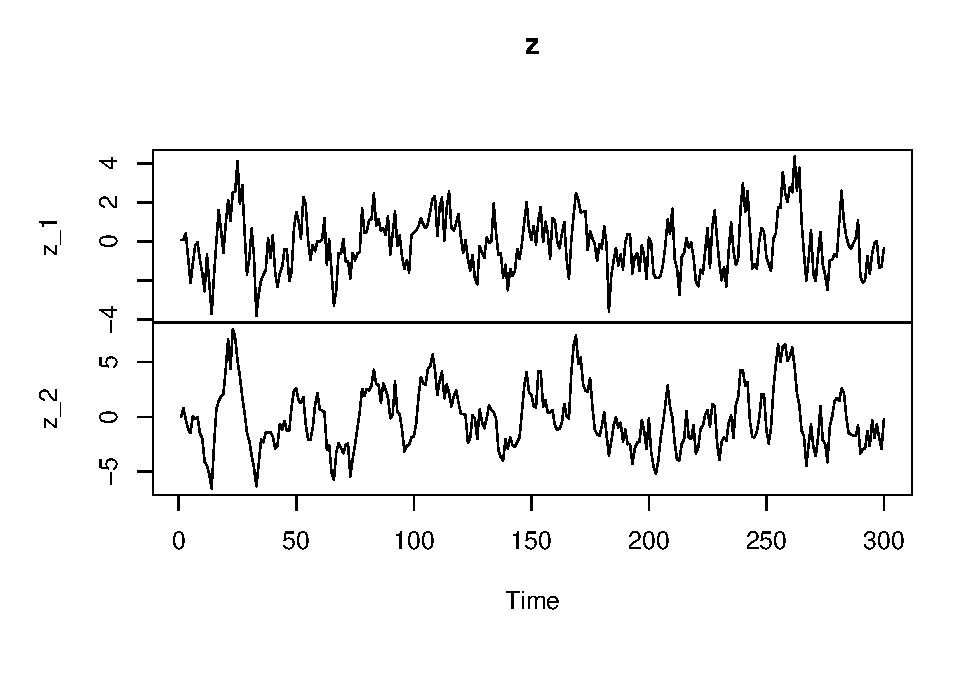
\includegraphics{exercise_2_files/figure-latex/unnamed-chunk-8-1.pdf}

At least it looks stable hence we cannot rule out stationarity.

\begin{itemize}
  \item[e)] Estimate the sample cross-covariance and cross-correlation matrices. Compare these with the population moment matrices from task a)
\end{itemize}

\begin{align*}
  \widehat{\Gamma_0} & = \tilde{z}_T^{'} \tilde{z}_{T-1} \cdot (T - 1)^{-1} \\
  \tilde{z}_T^{'} & = z_T - \widehat{\mu}_z\\
  Z & \ \text{is a} \ T \times 2 \ \text{matrix}\\
  z_t &\  \text{is a} \ 2 \times 1 \ \text{vector}\\
  z_t & := 
  \begin{pmatrix}
    x_t \\
    y_t
  \end{pmatrix} \; \leftarrow \text{variables}\\
  Z_t & := 
  \begin{pmatrix}
    X_{t} & Y_{t} \\
    X_{t-1} & Y_{t-1} \\
    X_{t-2} & Y_{t-2} \\
    \vdots & \vdots \\
    X_{t-t} & Y_{t-t} \\
  \end{pmatrix} \; \leftarrow \text{sample data}\\
\end{align*}

\begin{align*}
  \widehat{\Cov(x_t, y_{t-1})}
\end{align*}

\end{document}
